\documentclass{beamer}
 
\usepackage[utf8]{inputenc}
\usepackage{amsmath}
\usepackage{tabto}
\usepackage{graphicx}
\usepackage{newtxmath}
\usepackage{bm}
 
%Information to be included in the title page:

\usetheme{Copenhagen}
\title[Simplex] %optional
{EE5327 Optimization}
 
 
\author[Anshika,Razat,Bhavani] % (optional, for multiple authors)
{Anshika Chaurasia \and Razat Shanker \and Bhavani Machnoori}
 
\institute[VFU] % (optional)
{
  
  EE18MTECH11017\\
  EE18MTECH11016\\
  EE18ACMTECH11006
 
 }
 
\date[VLC 2013] % (optional)
{28 Feb 2019}
 
 
\begin{document}
 
\frame{\titlepage}

 
 \begin{frame}
 \frametitle{Question 51}
 
Q. Maximize
\begin{center}
    w = 11x - z 
\end{center}
 
 \\ with constraints
\begin{alignat*}{1}
 \\  10x + y - z &\le 1 
 \\  2x + 2y + z &\le 2 
 \\ \hspace{0.1cm} x,y,z &\ge 0
 \end{alignat*}
Then, the maximum value of w is equal to ......
\end{frame}
 
\begin{frame}
 \frametitle{Solution}
 
Adding slack variables s_{1} \ge 0,s_{2} \ge 0

\[ \\ 10x + y - z + s_{1} = 1
 \\ 2x - 2y + z + s_{2} = 2   \]   

Objective function f(x) = 11x + 0y - z + 0s_{1} + 0s_{2}
\end{frame}

\begin{frame}
 \frametitle{Solution}
 
\begin{center}
    Initial Simplex Table
\end{center}

    \begin{table}[!ht]
   \centering
   \begin{tabular}{|c|c|c|c|c|c|c|c|c|} \hline
     &C_{j} &11 &0 &-1 &0 &0 & &
     \\ &  &x &y &z &s_{1} &s_{2} &RHS &\theta  \\ \hline
      0 &s_{1} &  \textbf{10}  &1 &-1 &1 &0 &1 & $ \frac{\textbf{1}}{\textbf{10}} $ $\rightarrow$ \\ \hline
      0 &s_{2} &2 &-2 &1 &0 &1 &2 &1 \\ \hline
      &C_{j} - w_{j} &\textbf{11} $ \uparrow $ &0 &-1 &0 &0 &w_{RHS} = 0 & \\ \hline
     
     \end{tabular}
    \end{table} 
    x - Entering Variable 
  \\  $s_{1}$  - Leaving variable
   \\ 10 - pivot
\end{frame}

\begin{frame}
 \frametitle{Solution}
 
 \begin{columns}
  \begin{column}{0.47\textwidth}
 w_{1} = 
 \begin{pmatrix} 
0 \\ 
0 
\end{pmatrix}
.  
  \begin{pmatrix} 
10 \\ 
2 
\end{pmatrix}

\\   w_{2} = 
  \begin{pmatrix} 
0 \\ 
0 
\end{pmatrix}
.
  \begin{pmatrix} 
1 \\ 
-2 
\end{pmatrix}

  w_{3} = 
  \begin{pmatrix} 
0 \\ 
0 
\end{pmatrix}
.
  \begin{pmatrix} 
-1 \\ 
1
\end{pmatrix}

\\  w_{4} = 
  \begin{pmatrix} 
0 \\ 
0 
\end{pmatrix}
.
\begin{pmatrix} 
1 \\ 
0 
\end{pmatrix}

\\\\  w_{5} = 
  \begin{pmatrix} 
0 \\ 
0 
\end{pmatrix}
.
\begin{pmatrix} 
0 \\ 
1 
\end{pmatrix}
  \end{column}
  \begin{column}{0.63\textwidth}
    w_{RHS} = 
  \begin{pmatrix} 
0 \\ 
0 
\end{pmatrix}
.
\begin{pmatrix} 
1 \\ 
2 
\end{pmatrix}
\vspace{1cm}
\\
\theta = 
RHS Value \\ \hline
\hspace{0.7cm} Corresponding value in columns of x
  \end{column}
\end{columns}

  \end{frame}

\begin{frame}
 \frametitle{Solution}
 First iteration \\
  R_{1} $ \rightarrow $ \textstyle\frac{R_{1}}{10}
    \\ R_{2} $ \rightarrow $ R_{2} - 2R_{1}
    \\  R_{3} $ \rightarrow $ R_{3} - 11R_{1}
  \begin{table}[!ht]
   \centering
   \begin{tabular}{|c|c|c|c|c|c|c|c|c|} \hline
     &C_{j} &11 &0 &-1 &0 &0 & &  \\ \hline
      &  &x &y &z &s_{1} &s_{2} &RHS & \theta  \\ \hline
      11 &x &1  & $\frac{1}{10}$ \vspace{1mm} & $\frac{-1}{10}$ & $ \frac{1}{10} $ &0 &$\frac{1}{10}$ &- \\ \hline
      0 & \[s_{2}\] &0  & $\frac{-11}{5}$ \vspace{1mm}  & $\frac{\textbf{6}}{\textbf{5}}$ & $ \frac{-1}{5} $ &1 &$\frac{9}{5}$ & $\frac{3}{2}$ $\rightarrow$ \\ \hline
      &C_{j} - w_{j} &\textbf{11} $ \uparrow $ &0 &-1 &0 &0 &w_{RHS} = \frac{11}{10} & \\ \hline
     
     \end{tabular}
    \end{table}
    x - Entering Variable 
  \\  $s_{1}$  -  Leaving variable
  \\ $\frac{6}{5}$- Pivot
\end{frame}

\begin{frame}
 \frametitle{Solution}
 \vspace{1cm}
 Second iteration : \\
  R_{2} $ \rightarrow $ R_{2} x \frac{5}{6}
    \\ R_{1} $ \rightarrow $ R_{1} + \textstyle\frac{R_{2}}{10}
    \\  R_{3} $ \rightarrow $ R_{3} - \textstyle\frac{R_{2}}{10}
  \begin{table}[!ht]
   \centering
   \begin{tabular}{|c|c|c|c|c|c|c|c|} \hline
     &C_{j} &11 &0 &-1 &0 &0 &   \\ \hline
      &  &x &y &z &s_{1} &s_{2} &RHS   \\ \hline
      11 &x &1  & $\frac{-1}{12}$  &0 & $ \frac{1}{10} $ &$\frac{1}{12}$ &$\frac{1}{4}$ \vspace{1mm}  \\ \hline
     --1  &z &0  & $\frac{-11}{6}$ \vspace{1mm} &1 & $ \frac{-1}{6} $  &$\frac{5}{6}$ & $\frac{3}{2}$  \\ \hline
      &C_{j} - w_{j} &0 &$\frac{-11}{12}$ &0 &$\frac{-13}{12}$ &$\frac{-1}{12}$ &w_{RHS} = \frac{5}{4}  \vspace{1mm} \\ \hline
     
     \end{tabular}
    \end{table}
 Here all $C_{j} - w_{j}$ values are either zero or negative. \\So, maximum value of w = w_{RHS} =  \frac{5}{4} \\ for x = $\frac{1}{4}$ and z = $\frac{3}{2}$.  
\end{frame}

\begin{frame}
\frametitle{Question 51}
Q. Use cvxopt to obtain a solution to problem 51.  
 \begin{center}

 $\min\limits_{x}\ c^Tx$
\begin{alignat*}{2}
  \\subject\hspace{0.1cm} to\hspace{0.1cm}  Ax &\preceq b
\end{alignat*}

\end{center}
\[
c = 
\begin{bmatrix}
-11 
\\0
\\1
\end{bmatrix}
,A = 
\begin{bmatrix}
1  & 1 & -1
\\2  & -2 & 1
\\-1  & 0 & 0
\\0  & -1 & 0
\\0 & 0 & -1
\end{bmatrix}
,B = 
\begin{bmatrix}
1
\\2 
\\0 
\\0
\\0
\end{bmatrix}
\]
\end{frame}

\begin{frame}
\frametitle{Solution}
\begin{block}{Code:}

from cvxopt import matrix, solvers \vspace{0.5cm}

\\ A = matrix([ [10.0, 1.0,-1.0],
            [2.0, -2.0, 1.0],
            [-1.0, 0.0, 0.0],
 \\ \hspace{2cm}         [0.0, -1.0, 0.0], 
            [0.0, 0.0, -1.0]  ])
\\ b = matrix([ 1.0, 2.0, 0.0, 0.0, 0.0])
\\ c = matrix([ -11.0, 0.0, 1.0 ])

\\ sol = solvers.lp(c, A.T, b)
\\ print(sol['x'])
\\ print("cost function=")
\\ print(-1 * np.dot(np.reshape(c,(1,3)),sol['x']))
 \end{block}
  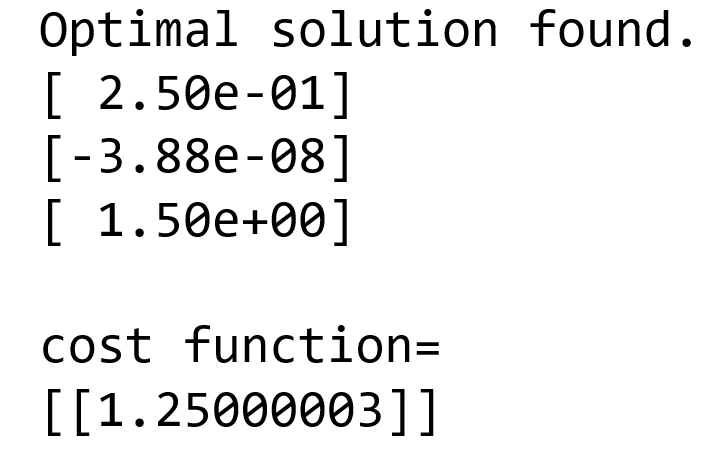
\includegraphics[width=4.5cm,height=2.5cm,angle=0]{Capture}
\end{frame}

\end{document}
